Le contenu des mini-jeux peut être très varié : jeu de rôle, jeu de gestion, jeu de plateforme, etc.
L'analyse des différences et des ressemblances entre ceux-ci, afin de définir ensuite une grammaire de description de jeux, est d'autant plus complexe.

Afin de nous confronter aux problèmes liés à l'implémentation de petits jeux vidéos et de faciliter l'analyse de la façon de décire un jeu, 
nous avons développé un échantillon de 8 types de mini-jeux en 2D dans le langage javascript.

Ces jeux n'ont pas été choisi par hasard : chacun possède un intérêt dans la description de ses règles et son implémentation.

\vspace{0.5cm}

\begin{tabular}{l|l}
 Jeu & Intérêt majeur \\
 \hline
 Pacman & ?? \\
 1942 & Vague d'ennemis \\
 Volley & Logique de score \\
 Course & Intelligence artificielle \\
 Mario & Niveaux \\
 Game\&Watch & ?? \\
 Billard & Collisions \\
 Jeu de Gestion & Ressources \\
\end{tabular}

\vspace{0.5cm}

Nous allons désormais présenter chacun de ces mini-jeux, pour ensuite analyser leurs objectifs, 
leurs règles et de façon plus générale leurs contenus afin d'en resortir différents aspects récurrents.

\subsection{Présentation des mini-jeux}

\note{c'est pour l'instant un bête copier coller de chacun, les fautes n'ont pas été corrigés.
On retravaillera cette sous-partie pour homogénéiser les différentes descriptions}

\subsubsection{Pacman}

Ce jeu est une adaptation du jeu classique de Pacman. 
Le joueur contrôle le TUX via les touches du clavier. 
Son but est de manger toutes les pommes sur le terrain tout en évitant les Microsoft qui essayent de l’attraper. 
Pour arriver a cet objectif, le joueur disposera de 3 vies. Le TUX pourra manger des pommes en or pour pouvoir détruire les Microsoft 
un petit temps et marquer quelques points en plus. En ce qui concerne l’affichage, le joueur verra le nombre de vie restante, 
son score ainsi que le temps ou les Microsoft restent vulnérables. Le Jeu est adaptable car il est facile d’initialiser 
la carte a partir d’images et d’un fichier Json.

\begin{figure}
 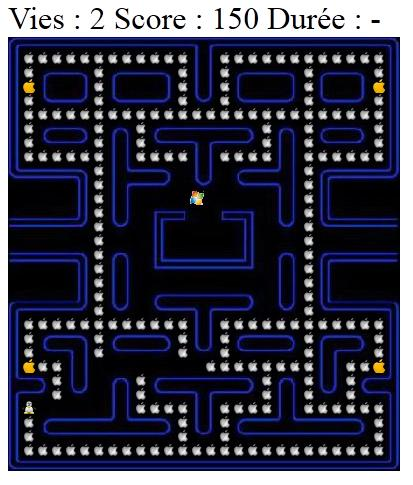
\includegraphics[width=\linewidth]{img/capturejeu_pacman}
 \caption{Capture du mini-jeu Pacman}
 \label{fig:game_pacman}
\end{figure}

\subsubsection{1942}

Dans ce shoot them up (jeu d’action où le joueur fait face à une multitude d’ennemis), 
le joueur contrôlera un vaisseau armé de deux canons pour détruire tous les véhicules adverses pour gagner des points. 
Le joueur aura 3 vies pour faire un maximum de point. Lorsque le joueur perd une vie, il devient invincible un petit moment pour reprendre la main ! 
Le vaisseau sera contrôlable via le clavier. En ce qui concerne les ennemis, ils suivent des déplacements prédéfinis qui peuvent être paramétrés. 
Le joueur n’est pas obligé de faire tuer tous les ennemis mais le but est quand même de faire le plus grand score !

\begin{figure}
 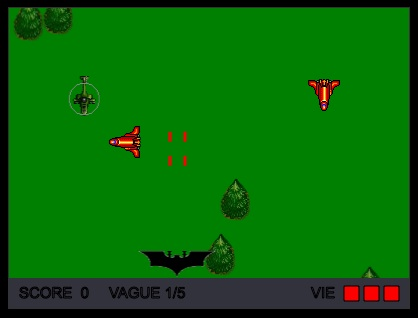
\includegraphics[width=\linewidth]{img/capturejeu_1942}
 \caption{Capture du mini-jeu 1942}
 \label{fig:game_1942}
\end{figure}

\subsubsection{Volley}


CowCow volley party  est un mini jeu humoristique mettant en scène deux vaches jouant au volley.
On peut jouer à ce jeu en mode solo avec une IA ou en multijoueur. 
Le but étant bien sur de gagner la partie en ayant 2 sets gagnants en premier. 
Pour cela votre vache dispose de 3 coups différents : passe courte et longue ainsi que le fameux smash !
Les règles de ce jeu sont les mêmes que les règles du volley classique. La vache sera contrôlée au clavier aussi bien  en mode multi qu’en mode solo.

\begin{figure}
 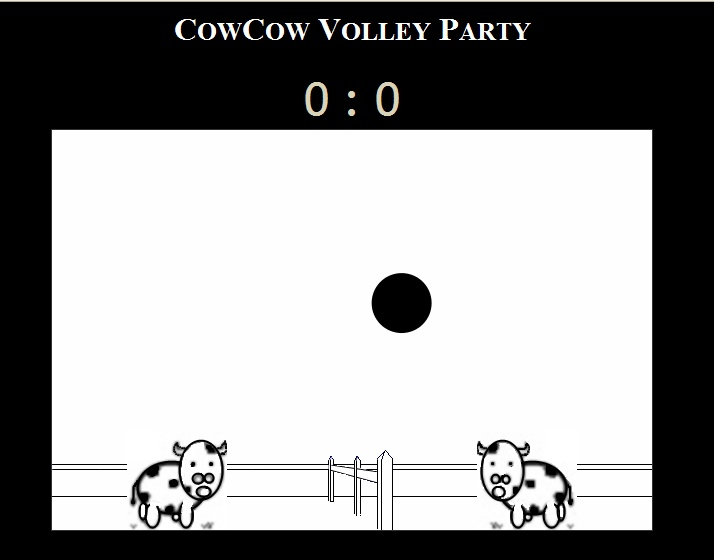
\includegraphics[width=\linewidth]{img/capturejeu_volleycowcow}
 \caption{Capture du mini-jeu volley}
 \label{fig:game_volley}
\end{figure}

\subsubsection{Course}

Ce jeu de course futuriste pour le web est un jeu pour un joueur qui se frottera à des intelligences artificielles pour faire le meilleur temps. 
Ce jeu de courses n’est pas un jeu de course classique, en effet sur le circuit vous trouverez des bonus 
(un turbo, un bonus permettant d’augmenter le temps d’un des autres joueurs, de changer leur positions, etc) 
et des zones de circuit différentes (inversion des commandes sur une zone, changement de vitesses, etc) 
ainsi que des objets fixes (turbo au sol,…). Vous pourrez choisir votre véhicule parmi une sélection de 12 vaisseaux différents. 
 En ce qui concerne les contrôles, le joueur se dirigera grâce à son clavier. Ce jeu est adaptable, il est, en effet, 
possible de créer facilement des circuits ainsi que des nouveaux bonus. Il serait aussi possible de mettre en place un système de 
lecture de fichier pour configurer les paramètres des différentes courses.

\begin{figure}
 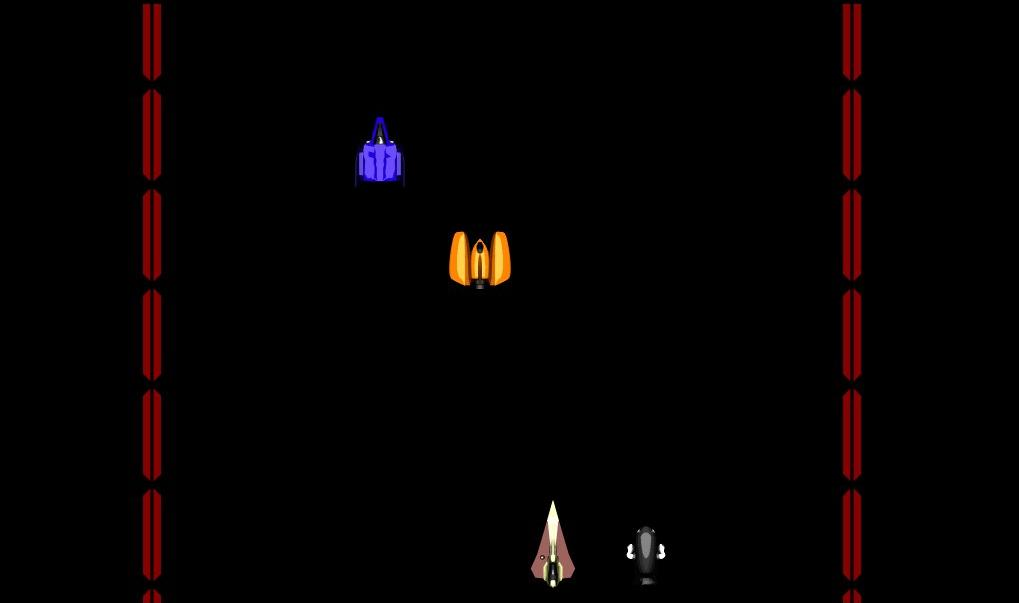
\includegraphics[width=\linewidth]{img/capturejeu_course}
 \caption{Capture du mini-jeu de course}
 \label{fig:game_course}
\end{figure}

\subsubsection{Mario}

Ce mini-jeu de plateforme reprend le principe des jeux du style de mario bros.
Un personnage, représenté par un rectangle, peut se déplacer sur les côtés ou sauter.
Il doit avancer au maximum, sans être touché par des ennemis, représentés par des triangles et sans tomber dans les trous du terrain.
Le personnage peut faire perdre des points de vie aux ennemis jusqu'à les tuer en leur sautant dessus. S'il les touche sur les côté, 
il meurt et la partie est terminée.
La caméra avance lorsque le joueur avance suffisamment. Le joueur peut revenir à gauche jusqu'à la limite de l'écran.
Le terrain est généré aléatoirement et est infini.
Le but du jeu est d'obtenir le plus grand score. Le score diminue avec le temps et augmente lorsqu'un ennemi est tué ou que le personnage avance

\subsubsection{Game \& Watch}

L’application est un mini-jeu du style Game \& Watch, où le personnage principal doit chasser ses ennemis avant que ces derniers ne l’atteignent.

Lors du jeu, les ennemis arrivent du bas de l’écran, et montent jusqu’à arriver au niveau du personnage, qui doit les écraser. S’il ne le fait pas, 
il perd une vie. A 0 vie, le jeu s’arrête et le joueur perd la partie.

Pour chaque ennemi écrasé, le joueur gagne un point déterminé de point. A partir d’un certain nombre de points qui sera définit plus tard, 
le jeu passe au niveau suivant, ce qui se traduit par l’augmentation de la difficulté, c’est-à-dire l’arrivée des ennemis s’accélère.

Lorsque le joueur arrive à détruire un de ses ennemis, il gagne un certains nombre de points. Par contre, lorsqu’un ennemi atteint le joueur, 
ce dernier perd une vie et son score reste intact.

Quand le joueur perd la partie, il doit pouvoir sauvegarder son score si ce dernier est dans les 5 meilleurs scores et si le joueur le souhaite.

Lorsqu’il ne reste au joueur que 2 vies, des vies “bonus” apparaissent pendant un certain temps, une à une, puis disparaissent; 
le joueur doit donc se déplacer vers elles pour les récupérer et augmenter ainsi son niveau de vie.

Les ennemis arrivent un par un du bas vers le haut, où se situe le joueur. 
La vitesse à laquelle ces ennemis arrivent est déterminée par le niveau actuel du jeu. 
Plus les niveaux augmentent plus la vitesse des ennemis s’accélère.

\begin{figure}
 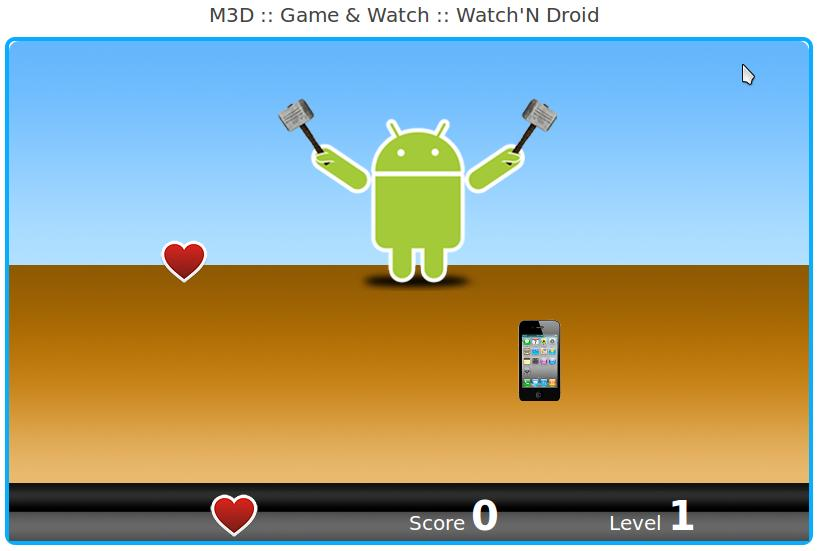
\includegraphics[width=\linewidth]{img/capturejeu_watchndroid}
 \caption{Capture du mini-jeu Game \& Watch}
 \label{fig:game_gamewatch}
\end{figure}

\subsubsection{Billard}

Ce mini-jeu de billard est un jeu multi-joueurs au tour par tour. 
Il reprend les règles classiques du billard anglais (chaque joueur doit rentrer toutes les boules d’une couleur puis la noire). 
D’un point de vue gameplay, le joueur contrôle la queue qui pointe automatiquement vers la boule blanche via sa souris. 
Le joueur peut ainsi choisir l’angle avec lequel il compte frapper la boule blanche et en fonction du pendant lequel le joueur va cliquer le tir va être plus ou moins fort. 
Pour l’affichage, chaque joueur voit combien de boules sont rentrés ainsi que sa couleur. Une icône verte apparait au niveau du joueur qui doit jouer. 
Le cadre bleu en bas de l’écran affiche la personne ayant gagné la partie !

\begin{figure}
 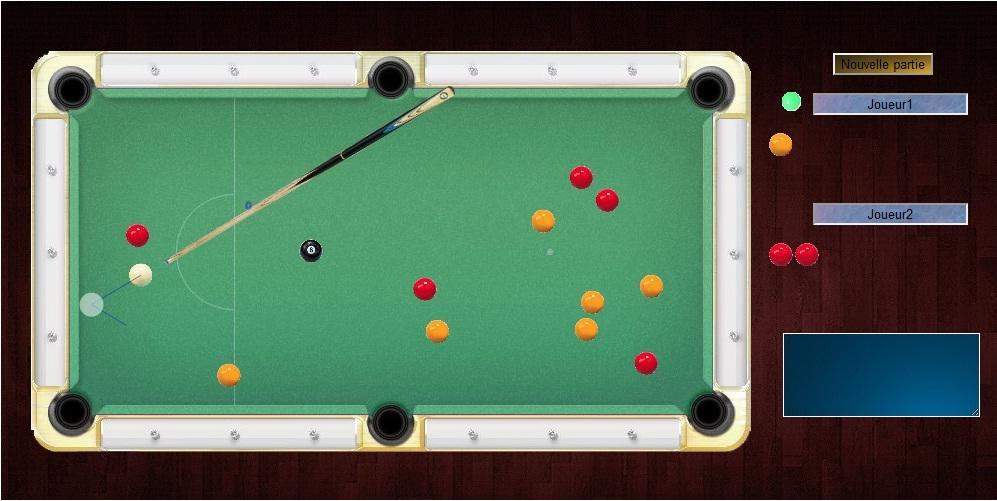
\includegraphics[width=\linewidth]{img/capturejeu_billard}
 \caption{Capture du mini-jeu billard}
 \label{fig:game_billard}
\end{figure}

\subsubsection{Gestion}

Le jeu commissariat est  un jeu de gestion du style Farmville. 
Vous aurez pour rôle de maintenir et améliorer votre commissariat en fonction des ressources disponibles.
 Les ressources sont au nombre de quatre : le nombre de policier, l’argent, l’indice IGPN et l’alcool ! 
Il y a trois actions disponibles pour le joueur. Il peut envoyer des policiers en missions dans un quartier 
choisis pour ramener de l’argent ainsi qu’un prisonnier.  Si un prisonnier est ramené, le joueur a la possibilité 
de libérer le prisonnier contre de l’argent ou de le tabasser (avec un fort risque de pénalité). 
Il peut aussi acheter des équipements ainsi que de l’alcool avec son argent. L’alcool est une ressource qui diminue constamment, 
le joueur doit ton veiller a toujours en avoir pour ne pas perdre. Il peut aussi perdre avec un indice d’IGPN trop élevé, cet indice 
monte avec toutes les mauvaises actions (tabasser un prisonnier, etc.).

\begin{figure}
 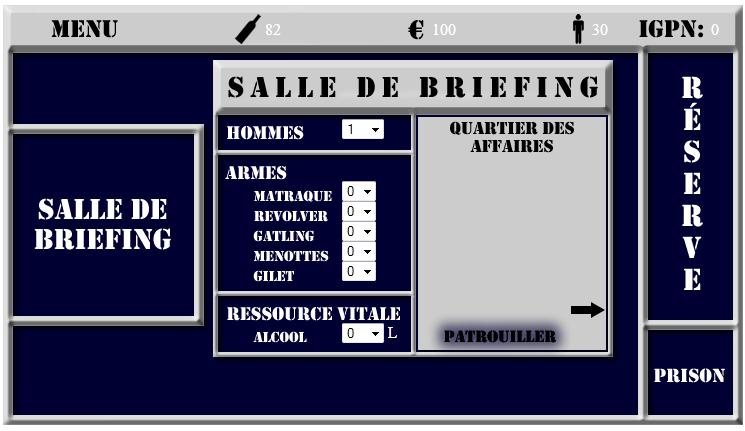
\includegraphics[width=\linewidth]{img/capturejeu_gestion2}
 \caption{Capture du mini-jeu de gestion}
 \label{fig:game_gestion}
\end{figure}

\subsection{Analyse des mini-jeux}

Suite au développement de ces mini-jeux, nous avons voulu analyser le contenu de ces différents jeux.
Pour cela, le tableau suivant récapitule différents aspects des jeux.

\note{inclure le tableau de google docs, en renvoyant peut être les colonnes pour mieux l'adapter à ce qu'on a fait dans la grammaire}

\vspace{0.5cm}

\begin{tabular}{|l|l}
\hline
 Jeu &   \\
\hline
 Pacman &  \\
\hline
 1942 &   \\
\hline
 Volley &  \\
\hline
 Course &  \\
\hline
 Mario &  \\
\hline
 Game\&Watch & \\
\hline
 Billard &  \\
\hline
 Jeu de Gestion & \\
\hline
\end{tabular}

\vspace{0.5cm}

Ce tableau permet de mieux identifier les différences et points communs entre les différents jeux.

On y voit par exemple que les objectifs au cours d'un niveau (ou pour un jeu sans niveau) revient souvent à atteindre une certaine zone
appelée ligne d'arrivée, ou éventuellement remplir des conditions de temps ou de ressources. En effet, à la fois la vie et le score
peuvent être vus comme une ressource : il s'agit d'un état, et une condition sur celui-ci est nécessaire à la victoire.
En faisant des conjonctions et des disjonctions de ces différentes possiblités, il est possible de définir 
les conditions de victoire pour tous les jeux (sauf le jeu de gestion).

En revanche, si on regarde comment le monde est construit, il est très différent d'un jeu à l'autre.
Pour certains comme Pacman, il est défini par une grille, pour d'autres comme le jeu de course, il est défini via un anneau.

Le tableau nous permet de voir assez clairement que le jeu de gestion est très différent des autres jeux.
Nous avons donc décidé de ne pas prendre en compte ce type de jeux.
Nous allons donc essayé de tirer des points communs entre les autres jeux, pour définir des concepts qui seront détaillés dans 
les parties suivantes.
Retirer de notre grammaire les jeux de gestion n'empêchent pas de couvrir un nombre important de jeux.
Il serait possible par exemple de définir plusieurs grammaires, chacune couvrant une catégorie de jeux afin de pouvoir
créer plusieurs types de jeux. Ainsi on pourrait créer une autre grammaire spécialement pour les jeux de gestion.
De la même façon, il est difficile de trouver des points communs entre les 7 mini-jeux restants, et un jeu de rôle où par exemple le joueur
doit réaliser plusieurs quetes.
Cependant, nous nous sommes concentrés pour le moment sur une unique grammaire décrivrant les 7 mini-jeux.

\note{Lister les concepts trouvés}
